% Compact PGFPlots panel for sampled qldpc_43_4_5_cluster_variant40_cap7 BSC correction-class derivative.
% Requires \usepackage{pgfplots} and \pgfplotsset{compat=1.18}.
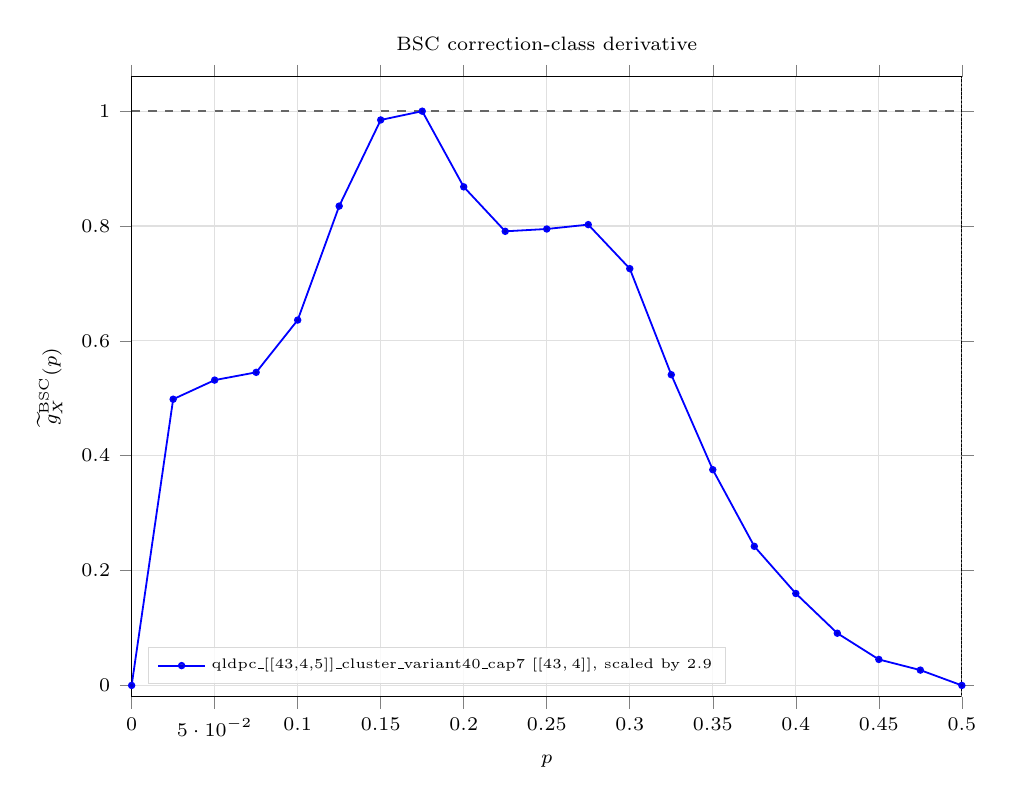
\begin{tikzpicture}
\begin{axis}[
  name=scaledBSCGEXITQldpc4345ClusterVariant40Cap7Axis,
  width=\linewidth,
  height=0.78\linewidth,
  title={BSC correction-class derivative},
  title style={font=\scriptsize},
  xlabel={$p$},
  ylabel={$\widetilde g_X^{\rm BSC}(p)$},
  xmin=0, xmax=0.5,
  ymin=-0.02, ymax=1.06,
  grid=both,
  major grid style={black!12},
  minor grid style={black!6},
  tick align=outside,
  tick label style={font=\scriptsize},
  label style={font=\scriptsize},
  legend cell align={left},
  legend style={draw=black!15, fill=white, fill opacity=0.82, text opacity=1, at={(0.02,0.02)}, anchor=south west, font=\tiny},
]
\addplot[black!60, densely dotted, line width=0.55pt, forget plot] coordinates {(0.5,-0.02) (0.5,1.06)};
\addplot[black!60, dashed, line width=0.55pt, forget plot] coordinates {(0,1) (0.5,1)};
\addplot+[color=blue, mark=*, mark size=1.0pt, line width=0.65pt]
coordinates {(0,0) (0.025,0.498405870662) (0.05,0.531699529119) (0.075,0.545213842483) (0.1,0.63621188988) (0.125,0.834760409352) (0.15,0.984717213222) (0.175,1) (0.2,0.86821143051) (0.225,0.790787600523) (0.25,0.794837194691) (0.275,0.80244509792) (0.3,0.725811606885) (0.325,0.541072587368) (0.35,0.375665506422) (0.375,0.24221979128) (0.4,0.160116465595) (0.425,0.0908900217599) (0.45,0.0452316243432) (0.475,0.0266688904745) (0.5,0)};
\addlegendentry{qldpc\_[[43,4,5]]\_cluster\_variant40\_cap7 $[[43,4]]$, scaled by $2.9$}
\end{axis}
\end{tikzpicture}
